\section{Theoretical Analysis}
\label{sec:analysis}

In this section, the circuit shown in Figure~\ref{fig:rc} is analysed
theoretically, in terms of the voltages and current intensities of the various branches and components of the circuit.

For convenience and coherence purposes, we chose to number the nodes of this circuit in the same manner that they will be numbered in the modified circuit used in the simulation. This means that nodes with the same number are in equivalent positions in the two circuits and explains why some numbers are skipped in this original circuit (the modified circuit has more nodes). In section ----- these modifications will be properly explained.
The nodes and meshes used in the following calculations are identified in Figure~(\ref{fig:circuit_analysis}).

\begin{figure}[h] \centering
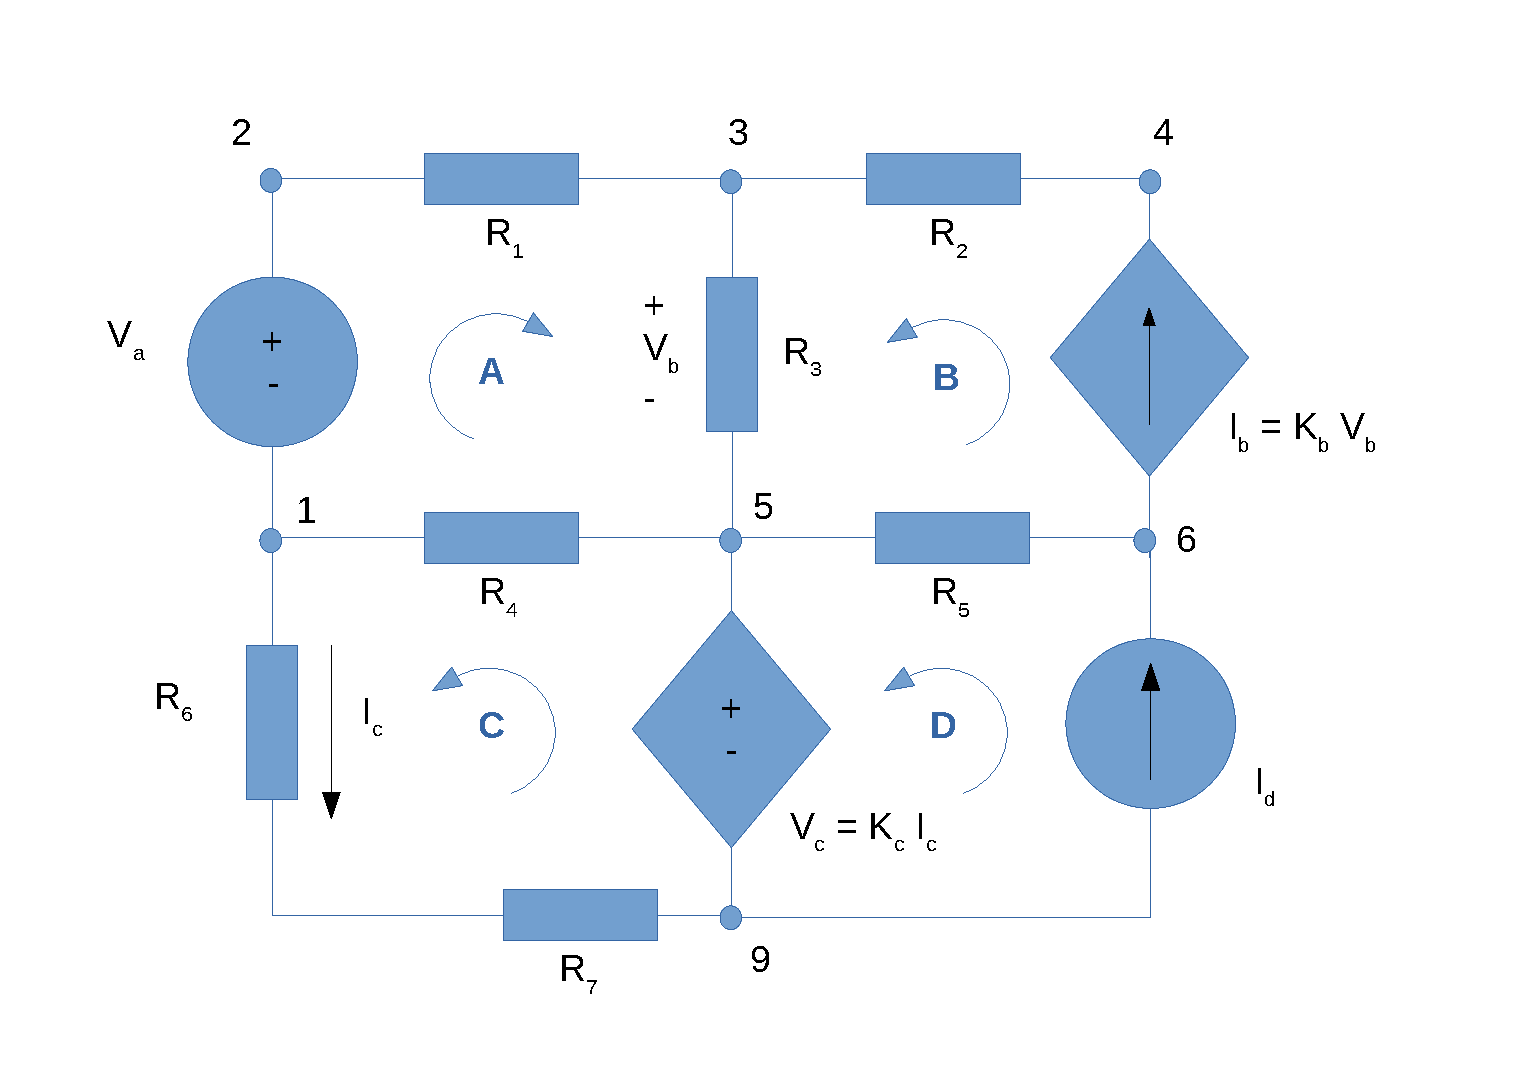
\includegraphics[width=0.8\linewidth]{circuit_analysis.pdf}
\caption{Circuit Nodes and Meshes Identification; nodes are identified by numbers and meshes are identified by capital letters; the circular arrows indicate de flow of the current that was arbitrarily chosen for each of the mesh's calculations.}
\label{fig:circuit_analysis}
\end{figure}


\subsection{Mesh Method}

The circuit consists of multiple loops with various values of current, $i$, circulating in each of its branches. There are two
voltage sources, $v_a$ and $v_c$, driving their inputs. Applying the Mesh Method, which in this case consists of identifying the KVL equations for meshes A and C, as well as any other necessary additional equations, we reached a system of 5 equations and 5 unkowns, that was solved using the Octave math tools. Those equations are:

\begin{equation}
  mesh a -> v_a - R_1*i_a - R_3*(i_a + i_b) - R_4*(i_a +i_c) = 0.
\end{equation}

\begin{equation}
  mesh c -> v_c - R_4*(i_a +i_c) - (R_6 +R_7)*i_c = 0.
\end{equation}

Additional equations:
$v_c = K_c*i_c$
$i_b = K_b*v_b$
$v_b = R_3*(i_a + i_b)$

The solution of this system of equations is presented in Table~(\ref{tab:node}). 

\begin{table}[h]
  \centering
  \begin{tabular}{|l|r|}
    \hline    
    {\bf Name} & {\bf Value [A or V]} \\ \hline
    Ia & 2.667112036144088e-01\\ \hline
Ib & -2.797307053897956e-01\\ \hline
Ic & 9.115165062107574e-01\\ \hline
Vb & -3.981339474096013e-02\\ \hline
Vc & 7.619521032756115\\ \hline

  \end{tabular}
  \caption{Table with the values of the unknowns from the system of equations obtained with the Mesh Method, solved using Octave; currents are expressed in Ampere and voltages are expressed Volts.}
  \label{tab:node}
\end{table}


\subsection{Nodal Method}

Another way of analysing the circuit is by applying the Nodal Method, which consists of identifying the FCL equations for the nodes not connected to a voltage source, as well as any other necessary additional equations. In this particular case, this means analysing nodes 3, 4 and 6, which led us to a system of 11 equations and 11 unknowns. After obtaining these equations, we repeated the previous procedure and solved the system with the Octave software. The equations obtained by applying this method are:


\begin{equation}
  node 3 -> (v_3 - v_5)*G_3 + (v_3 - v_2)*G_1 + (v_3 - v_4)*G_2 = 0.
  \label{eq:kvl}
\end{equation}

\begin{equation}
  node 4 -> (v_4 - v_3)*G_2 - i_b = 0.
\end{equation}

\begin{equation}
  node 6 -> i_b - i_d + (v_6 - v_5)*G_5 = 0.
  \label{eq:kvl2}
\end{equation}

Additional equations:
$v_1= 0$
$v_2 - v_1 = v_a$
$v_3 - v_5 = v_b$
$v_5 - v_9 = v_c$
$i_b = K_b*v_b$
$v_c = K_c*I_c$
$v_9 - v_1 = -i_c*(r_6 + r_7)$
$node 1 -> (v_2 - v_3)*G_1 + i_c +(v_1 - v_5)*G_4 = 0$

The solution of this system of equations is presented in Table~(\ref{tab:nodal}). 

\begin{table}[h]
  \centering
  \begin{tabular}{|l|r|}
    \hline    
    {\bf Name} & {\bf Value [A or V]} \\ \hline
    V0 & 0\\ \hline
V2 & 5.064003203930000\\ \hline
V3 & 4.796768408845987\\ \hline
V4 & 4.214279780392698\\ \hline
V5 & 4.836581803586947\\ \hline
V6 & 8.782125497855164\\ \hline
V9 & -2.782939229169170\\ \hline
Ib & -2.797307053897955e-01\\ \hline
Ic & 9.115165062107577e-01\\ \hline
Vb & -3.981339474096013e-02\\ \hline
Vc & 7.619521032756118\\ \hline

  \end{tabular}
  \caption{Table with the values of the unknowns from the system of equations obtained with the Nodal Method, solved using Octave; currents are expressed in Ampere and voltages are expressed Volts.}
  \label{tab:nodal}
\end{table}




